\section{FireBase}
\subsection{Concepts généraux}

\subsubsection{Définitions}

\textbf{Définition 01:} Firebase est une plateforme mobile créée en 2011 par James Tamplin et Andrew Lee \footnote{\textbf{James Tamplin et Andrew Lee :} les fondateur de Firebase, ils ont construits une société appelée Envolve, qui offrait des outils de discussion en temps réel sous forme de widgets pouvant être intégrés à un site Web} 4 sous le nom d'Envolve, puis rachetée par Google en 2014 pour être intégrée a leur offre de services Cloud (Google Cloud Platform). Son objectif premier est de libérer les utilisateurs de la complexité de création et de la maintenance d'une architecture serveur, tout en garantissant une scalabilite a toute épreuve (plusieurs milliards d'utilisateurs) et une simplicité dans l'utilisation.

\begin{figure}[h]
	\centering
    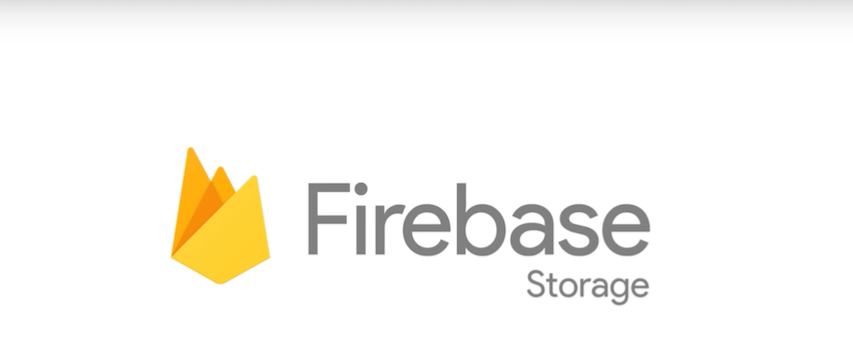
\includegraphics[scale=0.6]{img/part2/3.1}
    \caption{Logo FireBase}
\end{figure}

\textbf{Définition 02:} Firebase est un ensemble de services d'hébergement pour n'importe quel type d'application (Android, iOS, Javascript, Node.js, Java, Unity, PHP, C++ ..). Il propose d'héberger en NoSQL et en temps réel des bases de données, du contenu, de l'authentification sociale (Google, Facebook, Twitter et Github), et des notifications, ou encore des services, tel que par exemple un serveur de communication temps réel.

\subsubsection{Les produits de Firebase}

Firebase est conçu dans le but de libérer les utilisateurs de la complexité de création et de la maintenance d'une architecture serveur, tout en garantissant une scalabilite a toute épreuve (plusieurs milliards d'utilisateurs) et une simplicité dans l'utilisation. 

Pour cela, Firebase a été décomposée en plusieurs produits extrêmement riches et
adaptés au monde du mobile dont nous allons citer quelques uns.

\begin{itemize}

\item \textbf{Cloud Firestore :} Base de données NoSQL orientée documents de Firebase, permettant de facilement stocker, synchroniser et récupérer des données distantes pour une application mobile.

\item \textbf{Storage :} Espace de stockage de Firebase dédié au stockage et a la récupération de fichiers propres a l'utilisateur comme des photos ou des vidéos.

\item \textbf{Authentication :} Solution permettant de créer et gérer facilement des moyens d'authentification variés (Google, Facebook, Email, etc...) dans le but de sécuriser l'accès a une application mobile et authentifier les utilisateurs.

\item \textbf{Cloud Messaging :} Fournit un flux de communication fiable et économe en batterie entre le serveur (Firebase) et les appareils distants (ou l'application est installée) dans l'objectif d'envoyer et recevoir des messages de notifications.

\end{itemize}

\begin{figure}[h]
	\centering
    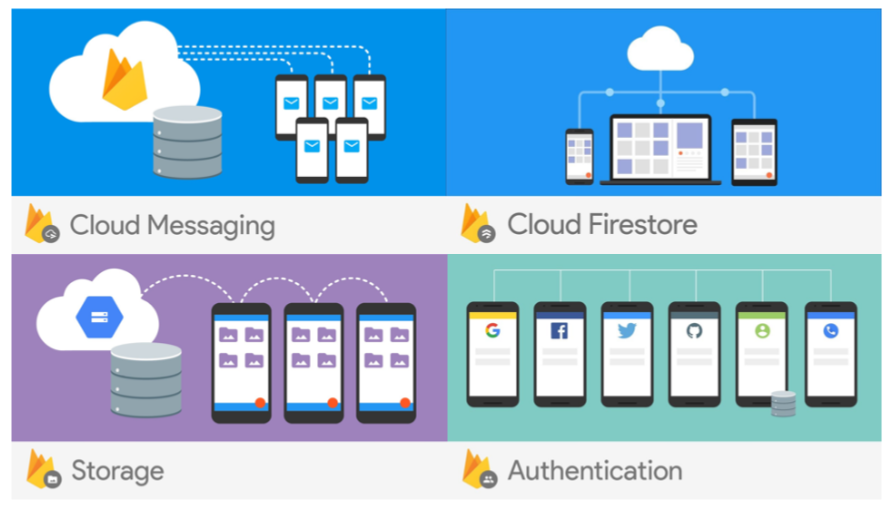
\includegraphics[scale=0.6]{img/part2/3.2}
    \caption{Quelques produits Firebase.}
\end{figure}